\documentclass[10pt]{beamer}
\usepackage[T1]{fontenc}
\usepackage[utf8]{inputenc}

\graphicspath{{}{figures/}}

\usetheme[progressbar=frametitle]{metropolis}
\usepackage{appendixnumberbeamer}

\usepackage{booktabs}
\usepackage[scale=2]{ccicons}

\usepackage{pgfplots}
\pgfplotsset{compat=1.12}
\usepgfplotslibrary{dateplot}

\usetikzlibrary{calc,fit,patterns}
\usepackage[absolute,overlay]{textpos}

\usepackage{xspace}
\newcommand{\themename}{\textbf{\textsc{metropolis}}\xspace}

\usepackage{xcolor}
\usepackage{listings}
\lstset{columns=fullflexible}
\lstdefinelanguage{EOL}{
morekeywords={delete,import,for,while,in,and,or,self,operation,return,def,var,throw,if,new,else,transaction,abort,
break,breakAll,continue,assert,assertError,not, switch, case, default},
sensitive=true,
morecomment=[l]{//},
morecomment=[l]{--},
morecomment=[s]{/*}{*/},
morecomment=[s]{-*}{*-},
morestring=[b]",
morestring=[b]',
showstringspaces=false
}

\lstnewenvironment{java}{\lstset{language=Java,
		frame=tb,
        tabsize=3,
        morekeywords={implies, in, result},
        basicstyle=\footnotesize,
        keywordstyle=\bfseries,
        ndkeywordstyle=\bfseries,
        commentstyle=\itshape,
		morecomment=[l]{--},
        stringstyle=\ttfamily,
		showspaces=false,
        flexiblecolumns,
        literate={->}{$\to$}{2} {--}{-$\,$-}{2} {<=}{$\le$}{2} {>=}{$\ge$}{2} {<>}{$<\,>$}{3},
        sensitive, extendedchars, texcl}}{}

\lstnewenvironment{ocl}{\lstset{language=[decorative]OCL,
	frame=tb,
	tabsize=3,
	morekeywords={implies,result,flatten,body,init,OrderedSet,Tuple,TupleType,def,attr,oclIsUndefined,oclIsInvalid,OclState,let,in},
	basicstyle=\footnotesize,
	keywordstyle=\bfseries,
	ndkeywordstyle=\bfseries,
	commentstyle=\itshape,
	stringstyle=\ttfamily,
	showspaces=false,
	flexiblecolumns,
	literate={->}{$\to$}{2} {--}{-$\,$-}{2} {<=}{$\le$}{2} {>=}{$\ge$}{2} {<>}{$<\,>$}{3},
	sensitive, extendedchars, texcl}}{}


\lstdefinelanguage{gremlin}{
morekeywords={as,def,fill,filter,groupCount,has,idx,inE,inV,is,label,length,match,outE,outV,v,values},
sensitive=true,
morecomment=[l]{//}
}

% "page cs" coordinate system
% From http://tex.stackexchange.com/questions/89588/
%
% Defining a new coordinate system for the page:
%
% --------------------------
% |(-1,1)    (0,1)    (1,1)|
% |                        |
% |(-1,0)    (0,0)    (1,0)|
% |                        |
% |(-1,-1)   (0,-1)  (1,-1)|
% --------------------------
\makeatletter
\def\parsecomma#1,#2\endparsecomma{\def\page@x{#1}\def\page@y{#2}}
\tikzdeclarecoordinatesystem{page}{
    \parsecomma#1\endparsecomma
    \pgfpointanchor{current page}{north east}
    % Save the upper right corner
    \pgf@xc=\pgf@x%
    \pgf@yc=\pgf@y%
    % save the lower left corner
    \pgfpointanchor{current page}{south west}
    \pgf@xb=\pgf@x%
    \pgf@yb=\pgf@y%
    % Transform to the correct placement
    \pgfmathparse{(\pgf@xc-\pgf@xb)/2.*\page@x+(\pgf@xc+\pgf@xb)/2.}
    \expandafter\pgf@x\expandafter=\pgfmathresult pt
    \pgfmathparse{(\pgf@yc-\pgf@yb)/2.*\page@y+(\pgf@yc+\pgf@yb)/2.}
    \expandafter\pgf@y\expandafter=\pgfmathresult pt
}
\makeatother
% Draws a grid for easier referencing of page cs values
\newcommand{\printtikzpagegrid}{
  \tiny
  \begin{tikzpicture}[overlay,remember picture,every node/.style={inner sep=.1em,draw=black!20,fill=white}]
    \foreach \x in {0,...,9} {
      \foreach \y in {0,...,9} {
        \node at (page cs:0.\x,0.\y) {};
        \node at (page cs:0.\x,-0.\y) {};
        \node at (page cs:-0.\x,0.\y) {};
        \node at (page cs:-0.\x,-0.\y) {};
      }
    }
    \node at (page cs:0,0) {0,0};
    \node at (page cs:0.5,0.5) {.5,.5};
    \node at (page cs:0.5,-0.5) {.5,-.5};
    \node at (page cs:-0.5,0.5) {-.5,.5};
    \node at (page cs:-0.5,-0.5) {-.5,-.5};
    \node at (page cs:1,1) {1,1};
    \node at (page cs:1,-1) {1,-1};
    \node at (page cs:-1,1) {-1,1};
    \node at (page cs:-1,-1) {-1,-1};
  \end{tikzpicture}
  \normalsize
}

\title{Taming Large Models\\with Hawk and NeoEMF}
%\subtitle{A modern beamer theme}
\date{MoDELS'2018, 14--19 October 2018}
\author{A. García-Domínguez, D. S. Kolovos, K. Barmpis, G. Daniel, G. Sunyé}
%\institute{Center for modern beamer themes}
% \titlegraphic{\hfill\includegraphics[height=1.5cm]{logo.pdf}}

\begin{document}

\maketitle

\begin{frame}{Table of contents}
  \setbeamertemplate{section in toc}[sections numbered]
  \tableofcontents[hideallsubsections]
\end{frame}

\section{Introduction}

\begin{frame}{Who are we? --- Hawk team}
\centering

\begin{columns}
\column{.3\textwidth}
\centering
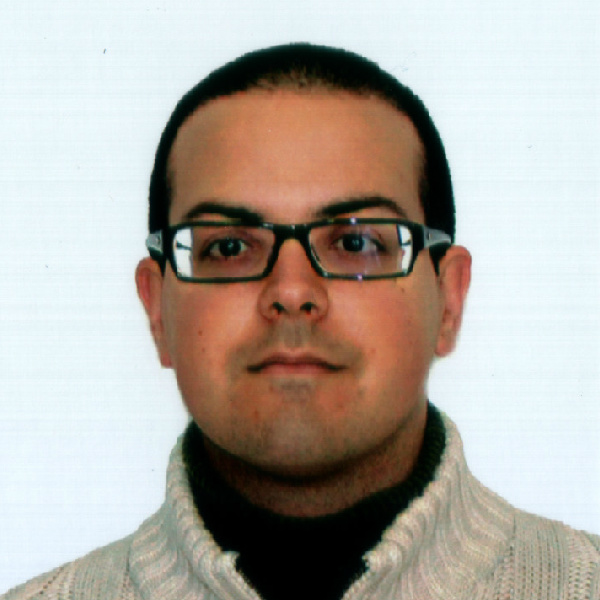
\includegraphics[height=.25\textheight]{biopic-01-antonio}
\column{.7\textwidth}
\begin{block}{Antonio (Lecturer, Aston University)}
\begin{itemize}
\item Hawk project lead
\item Eclipse Epsilon committer
\end{itemize}
\end{block}
\end{columns}

\begin{columns}
\column{.3\textwidth}
\centering
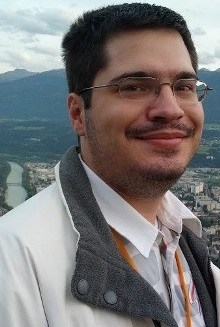
\includegraphics[height=.25\textheight,clip,trim={0 3cm 0 0}]{biopic-02-konstantinos}
\column{.7\textwidth}
\begin{block}{Konstantinos (Research Associate, U.\ of York)}
\begin{itemize}
\item Hawk initiator (core developer)
\item Created most core components
\end{itemize}
\end{block}
\end{columns}

\begin{columns}
\column{.3\textwidth}
\centering
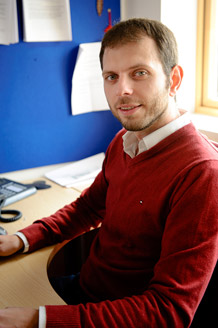
\includegraphics[height=.25\textheight,clip,trim={0 4cm 0 0}]{biopic-03-dimitris}
\column{.7\textwidth}
\centering
\begin{block}{Dimitris (Professor, University of York)}
\begin{itemize}
\item Hawk initiator (MONDO WP lead)
\item Eclipse Epsilon project lead
\end{itemize}
\end{block}
\end{columns}

\end{frame}

\begin{frame}{Who are we? --- NeoEMF team}

\begin{columns}
\column{.3\textwidth}
\centering
%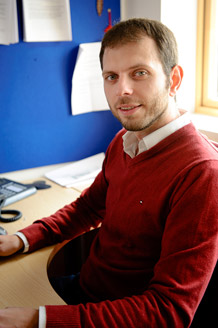
\includegraphics[height=.25\textheight,clip,trim={0 4cm 0 0}]{biopic-03-dimitris}
\column{.7\textwidth}
\centering
\begin{block}{Gwendal (Post-doc, SOM Research Lab)}
\begin{itemize}
\item NeoEMF core developer
\item Mogwaï project lead
\end{itemize}
\end{block}
\end{columns}

\begin{columns}
\column{.3\textwidth}
\centering
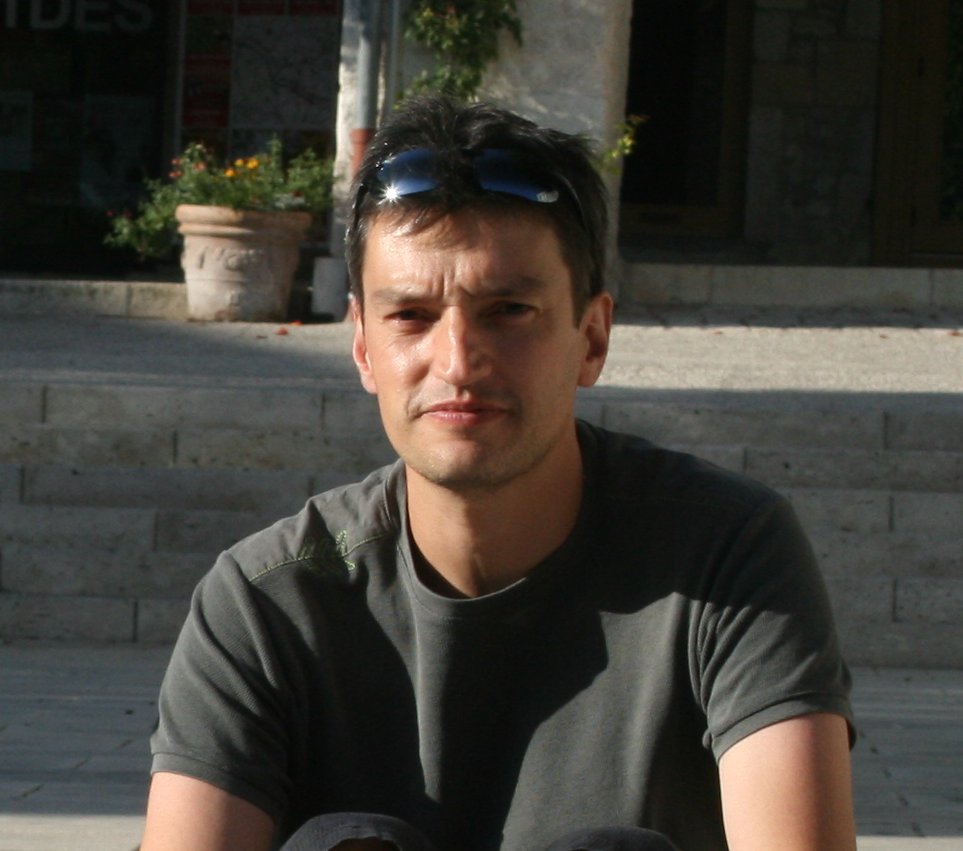
\includegraphics[height=.25\textheight,clip,trim={0 3cm 0 0}]{biopic-04-gerson}
\column{.7\textwidth}
\begin{block}{Gerson (Associate Professor, U.\ of Nantes)}
\begin{itemize}
\item NeoEMF initiator
\item AtlanMod project lead
\end{itemize}
\end{block}
\end{columns}

\end{frame}

\begin{frame}{Motivation: monolithic XMI models do not scale}
\centering

\begin{quote}
``[Lack of] Scalability is what is holding back a number of potential adopters''~\cite{Barmpis2013}
\end{quote}

\begin{quote}
``One can easily observe that scalability is the most critical of today's (and tomorrow's) challenges''~\cite{Mougenot2009}
\end{quote}

\begin{table}
\begin{tabular}{rrrr}
\toprule
Model & XMI (MB) & Avg.\ memory (MB) & Max memory (MB) \\
\midrule
%set0 & 8.75 & 22 & 49 \\
set1 & 26.59 & 53 & 135 \\
set2 & 270.12 & 437 & 840 \\
set3 & 597.67 & 849 & 1798 \\
set4 & 645.53 & 949 & 1910 \\
\bottomrule
\end{tabular}

\caption{Querying GraBaTs'09 Java models to find singletons}
\end{table}

\end{frame}

\begin{frame}{What to do?}

\begin{block}{Option 1: break up into fragments}
  \begin{itemize}
  \item Code is broken up into modules --- do the same with models
  \item Fragmented file-based models play well with traditional VCS
  \item Global queries may still require loading all fragments!
  \item \textbf{\alert{Hawk}} is our solution: indexes the fragments into a NoSQL database, queries the database instead of the fragments
  \end{itemize}
\end{block}

\begin{block}{Option 2: stop using files}
  \begin{itemize}
  \item Obviously not new: CDO has been doing it for years
  \item However, relational DBs are not the only option
  \item \textbf{\alert{NeoEMF}} can replace traditional XMI persistence with
    NoSQL approaches: graph databases, key-value stores...
  \end{itemize}
\end{block}

\end{frame}

\begin{frame}{Basic concepts about NoSQL}

\begin{block}{NoSQL = not only SQL}
  \begin{itemize}
  \item Generally, non-relational databases
  \item Some improve availability/performance by relaxing ACID
  \item Some are focused on specific analyses (e.g. social graphs)
  \end{itemize}
\end{block}

\begin{block}{Common types}
\begin{itemize}
\item \textbf{Key-value stores} implement an associative array to quickly fetch
  records given a tuple-based identifier (e.g. RocksDB, Redis).

\item \textbf{Document stores} keep collections of heterogeneous docs
  retrievable by key, supporting hierarchies + querying by field (e.g. MongoDB).

\item \textbf{Graph databases} store nodes, edges and their fields (e.g. Neo4j,
  OrientDB). Many support indexing and have query languages.

\item \textbf{Tuple stores} store subject-predicate-object triples (e.g. RDF4J,
  Jena). Very often used in Semantic Web approaches.
\end{itemize}
\end{block}

\end{frame}

\begin{frame}{Some considerations before we start}

  \begin{block}{NoSQL = purpose-specific databases}
    \begin{itemize}
    \item Can provide better capabilities than RDBMS, but require careful choice
      + benchmarking + tuning --- luckily, we did this for you :-)
    \item Technology/release/API all impact performance:
      \begin{itemize}
      \item Hawk Neo4j backend still in v2.0.5: later v2.x \emph{were slower},
        as Neo4j optimized for different requirements
      \item Hawk OrientDB v2.2.30 backend avoids \emph{slower} official OrientDB
        graph API, and uses the core document API instead
      \end{itemize}
    \end{itemize}
  \end{block}

  \begin{block}{Consider your requirements}
    \begin{itemize}
    \item Do you need faster queries?
    \item Do you need faster loading/saving? If so:
      \begin{itemize}
      \item Can you break up your files into fragments?
      \item Can you save to disk only the fragments that changed?
      \end{itemize}
    \end{itemize}

    We will revisit these during the wrap-up.
  \end{block}

\end{frame}

\section{Hawk}

\begin{frame}{Hawk: indexing for fast querying over fragment collections}
  \centering

  \begin{columns}[t]
    \column{.5\textwidth}
    \centering
    \begin{tikzpicture}[remember picture]
      \node (oldapproach) {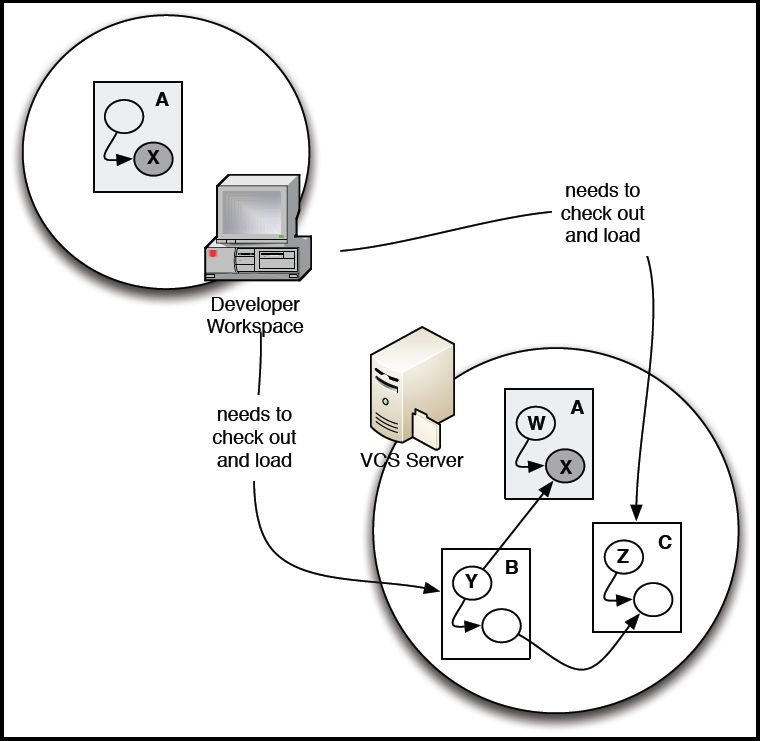
\includegraphics[width=\columnwidth,height=4.15cm,keepaspectratio]{old-approach}};
    \end{tikzpicture}
    \begin{block}{Usual approach}
      \begin{enumerate}
      \item Check out \textbf{all} files from VCS
      \item Load fragments into memory
      \item Run query (might go over all fragments)
      \end{enumerate}
    \end{block}

    \column{.5\textwidth}
    \centering
    \begin{tikzpicture}[remember picture]
      \node (newapproach) {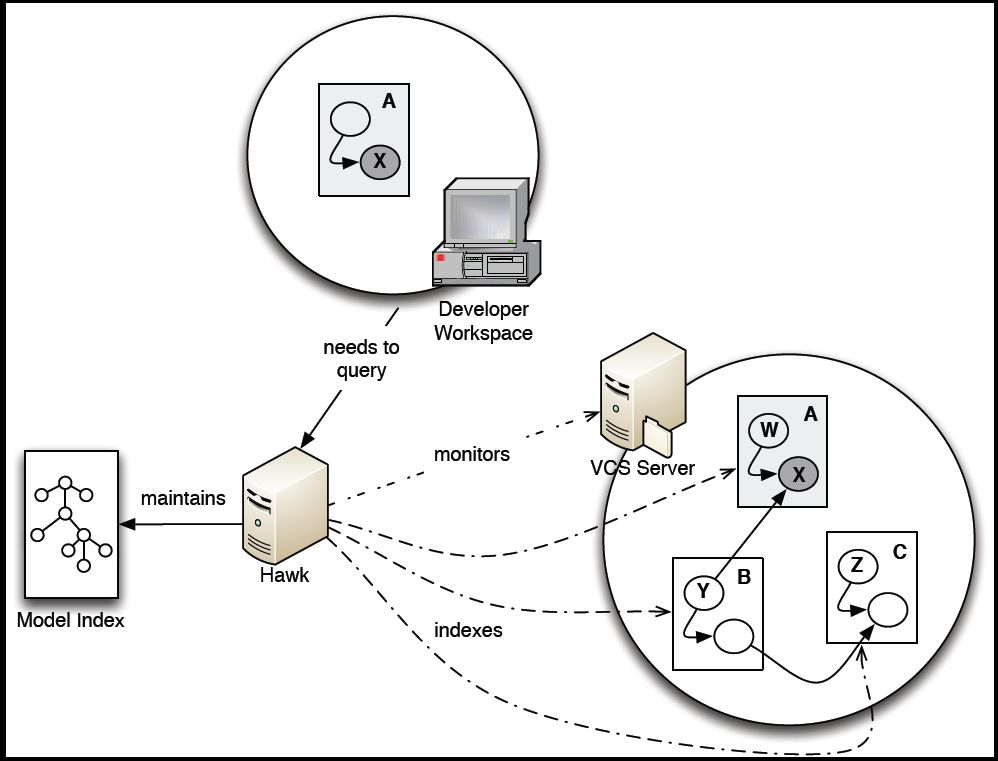
\includegraphics[width=\columnwidth,height=4.15cm,keepaspectratio]{hawk-approach}};
    \end{tikzpicture}
    \begin{block}{With Hawk}
      \begin{enumerate}
      \item Hawk watches VCS, indexes
      \item User queries Hawk over WS
      \item Hawk runs query through NoSQL database efficiently
      \item Hawk replies with result
      \end{enumerate}
    \end{block}

  \end{columns}

  \begin{tikzpicture}[overlay,remember picture]
    \draw[ultra thick,red,->] (oldapproach) -> (newapproach);
  \end{tikzpicture}
\end{frame}

\begin{frame}{Hawk: project website}
  \begin{center}
    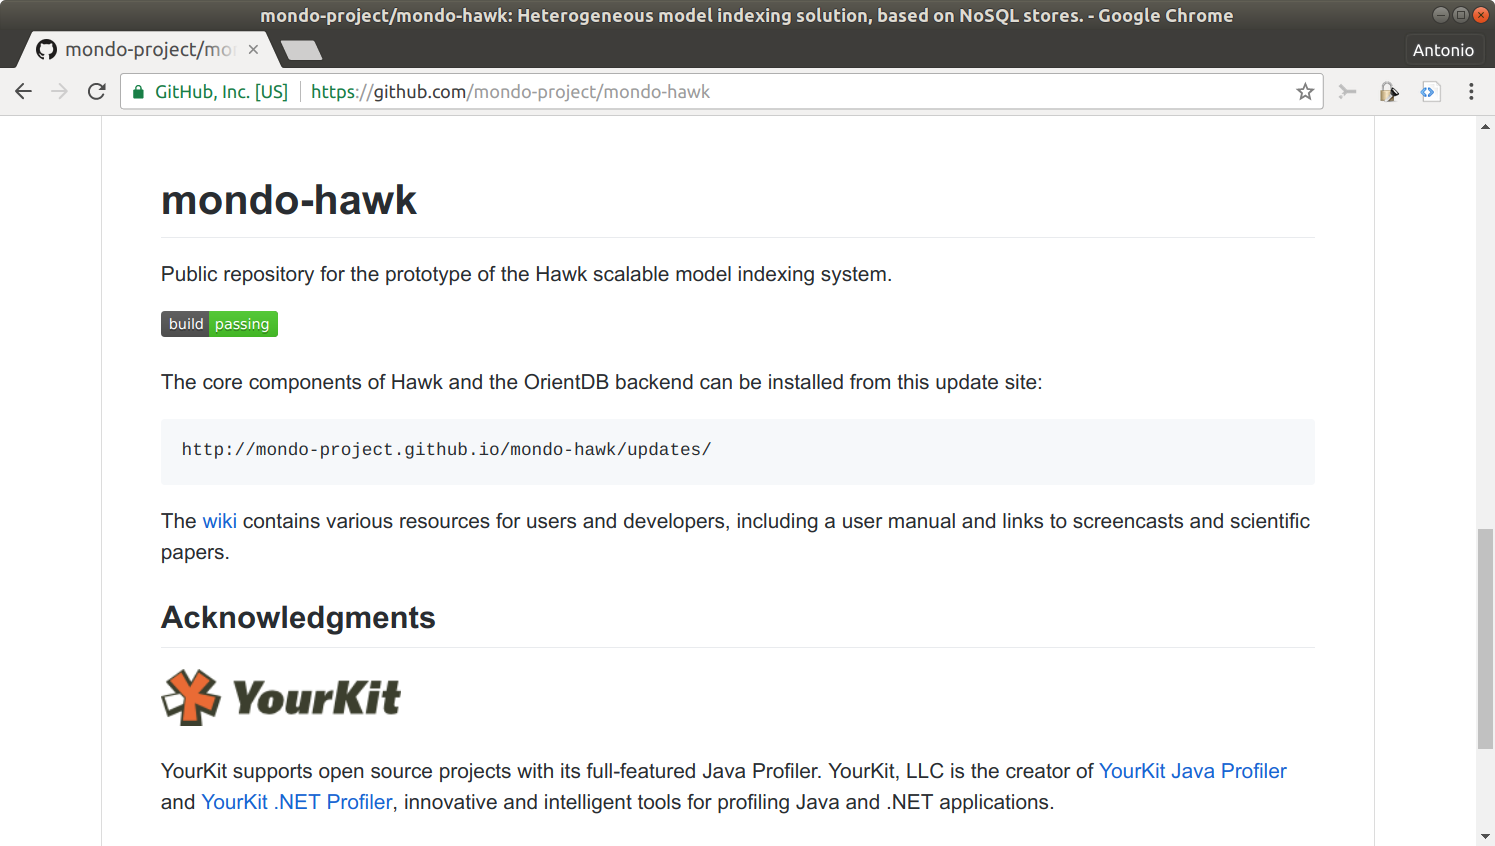
\includegraphics[width=\textwidth]{hawk-github}
  \end{center}

  \begin{itemize}
  \item \url{https://github.com/mondo-project/mondo-hawk}
  \item Open source project under the Eclipse Public License
  \end{itemize}
\end{frame}

\begin{frame}{Hawk: deployment}

  \begin{center}
    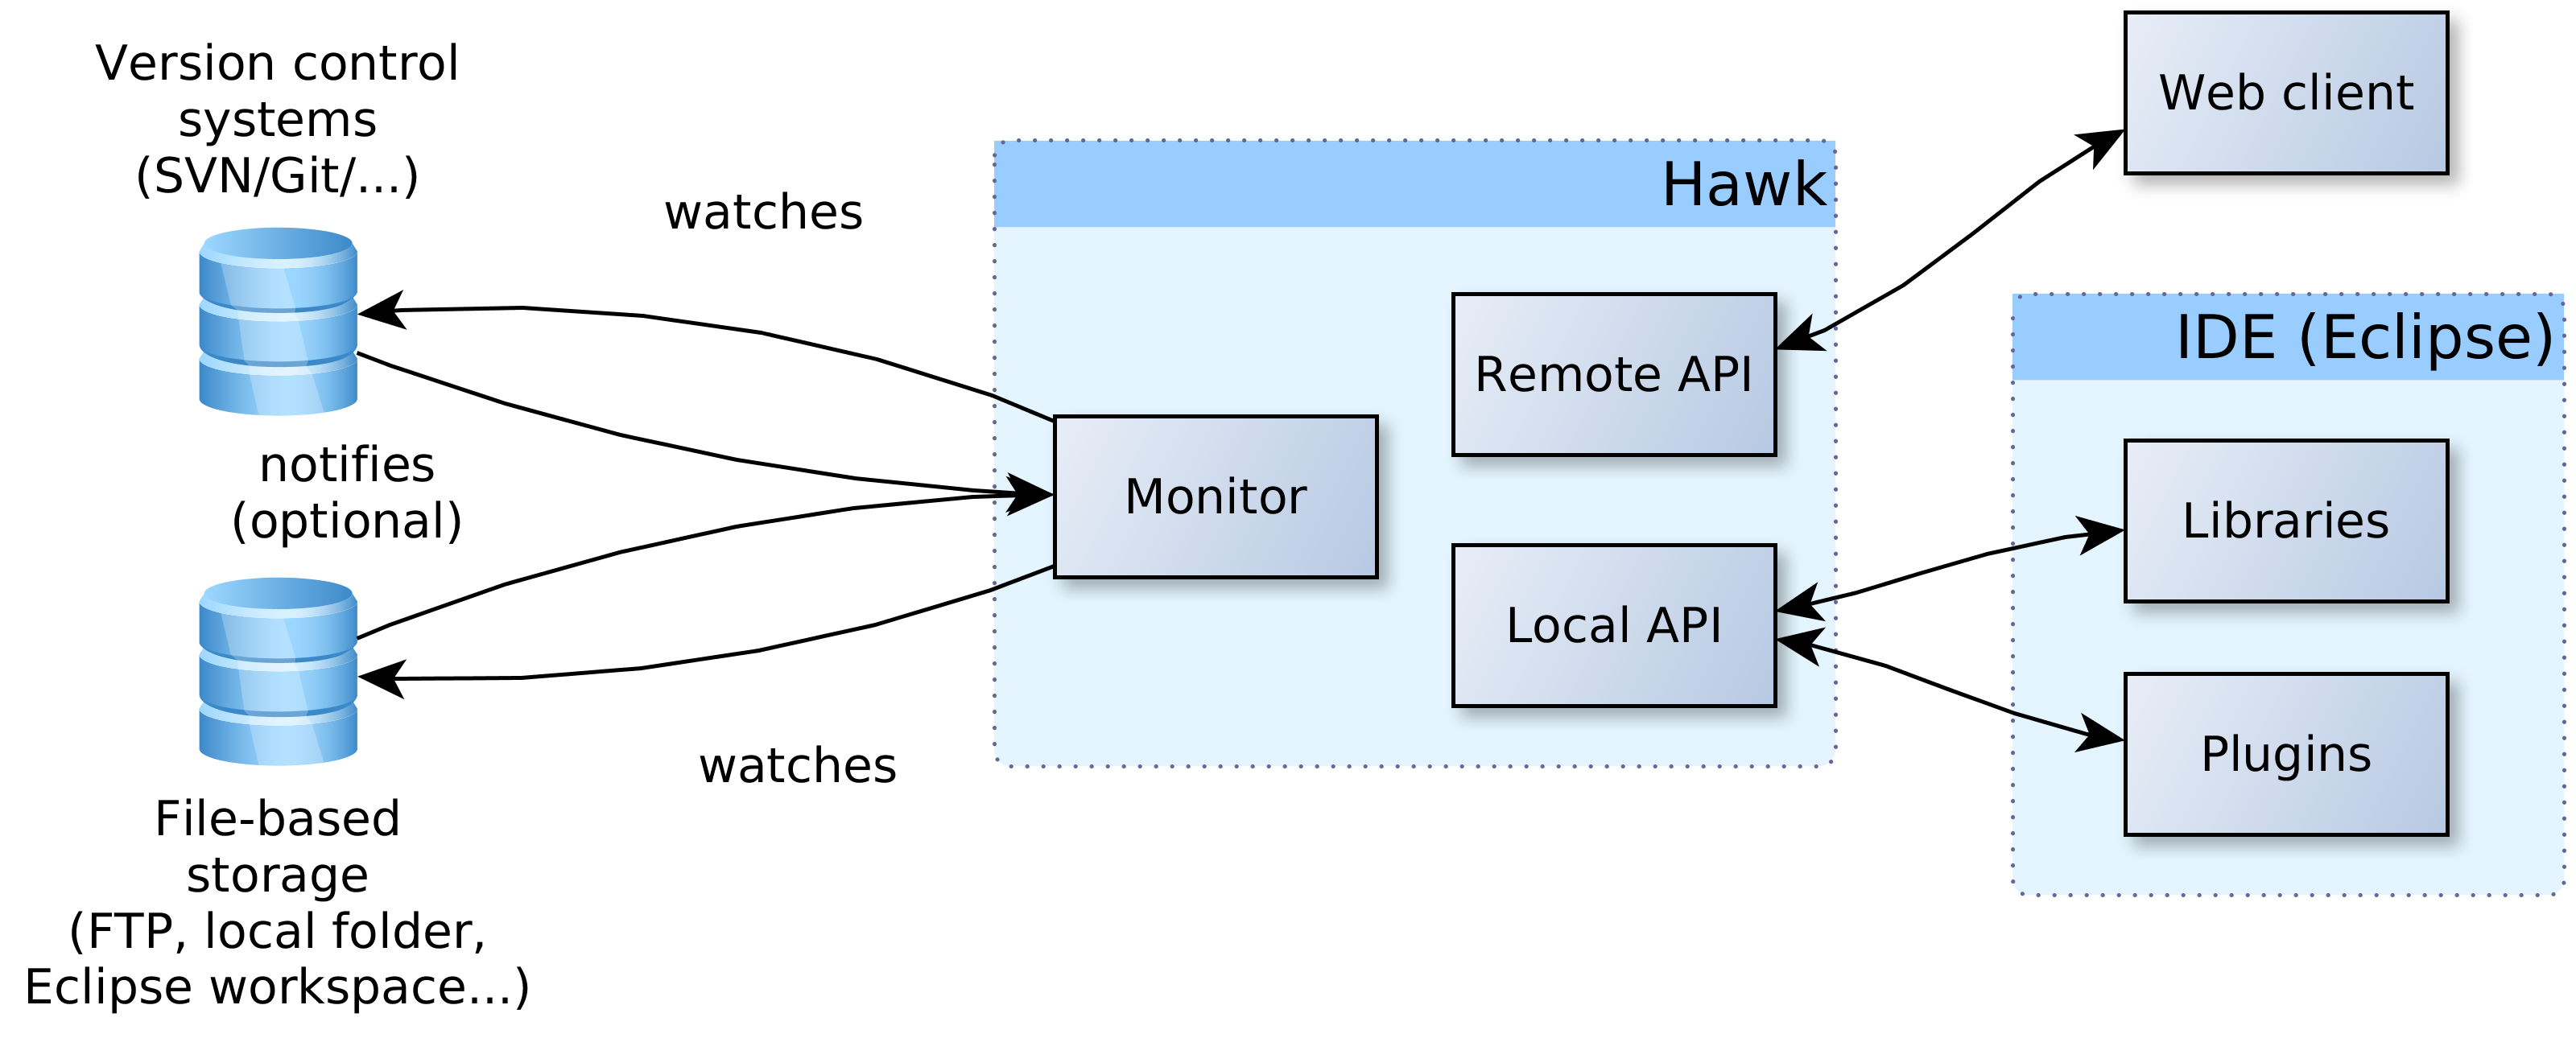
\includegraphics[width=\textwidth]{hawk-deployment}
  \end{center}

  \begin{itemize}
  \item Hawk can run as Eclipse plug-in, Java library, or network service
  \item We can have it watch over various types of locations:
    \begin{itemize}
    \item Version control systems (SVN/Git repositories)
    \item File stores (local folders, Eclipse workspaces, HTTP locations)
    \end{itemize}
  \end{itemize}

\end{frame}

\begin{frame}{Hawk: component-based architecture}
  \begin{center}
    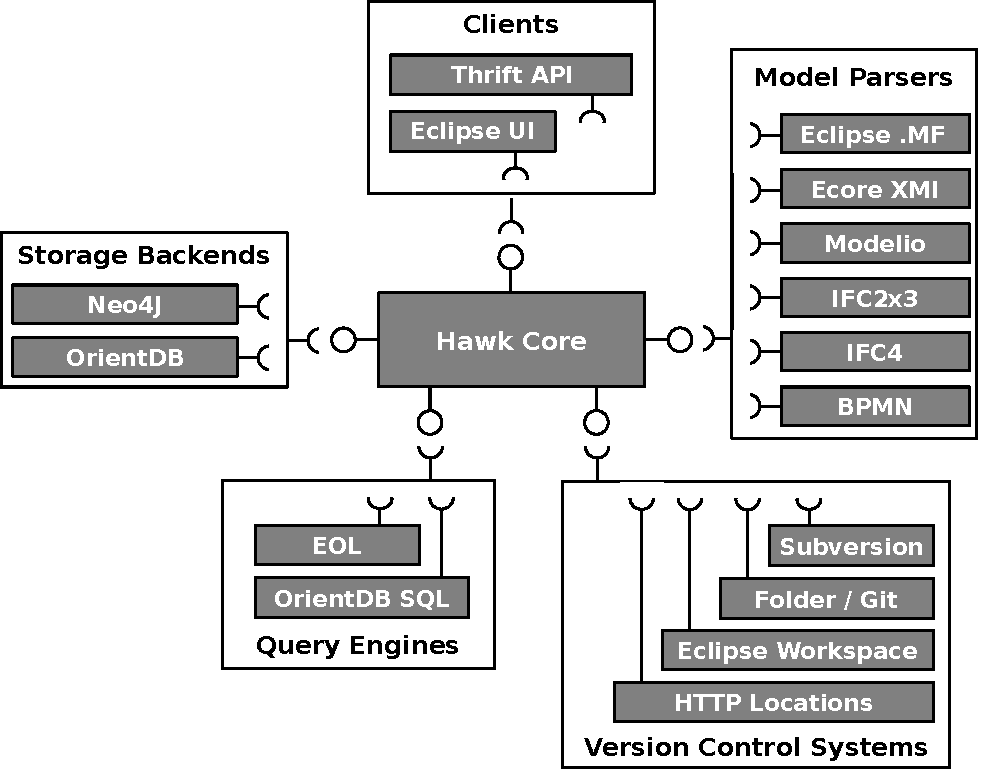
\includegraphics[width=.6\textwidth]{hawk-architecture}
  \end{center}

  \begin{itemize}
  \item Core: incremental graph updating + component interfaces
  \item Backends: Neo4j (fastest), OrientDB (multi-master), Greycat
  \item Clients: Eclipse GUI, cross-language Apache Thrift web services
  \item Query engines: Epsilon Object/Pattern Languages, OrientDB SQL
  \item Model parsers: EMF/Modelio models, Eclipse plug-in manifests...
  \end{itemize}
\end{frame}

\begin{frame}{Hawk: example for a library model}
  \centering
  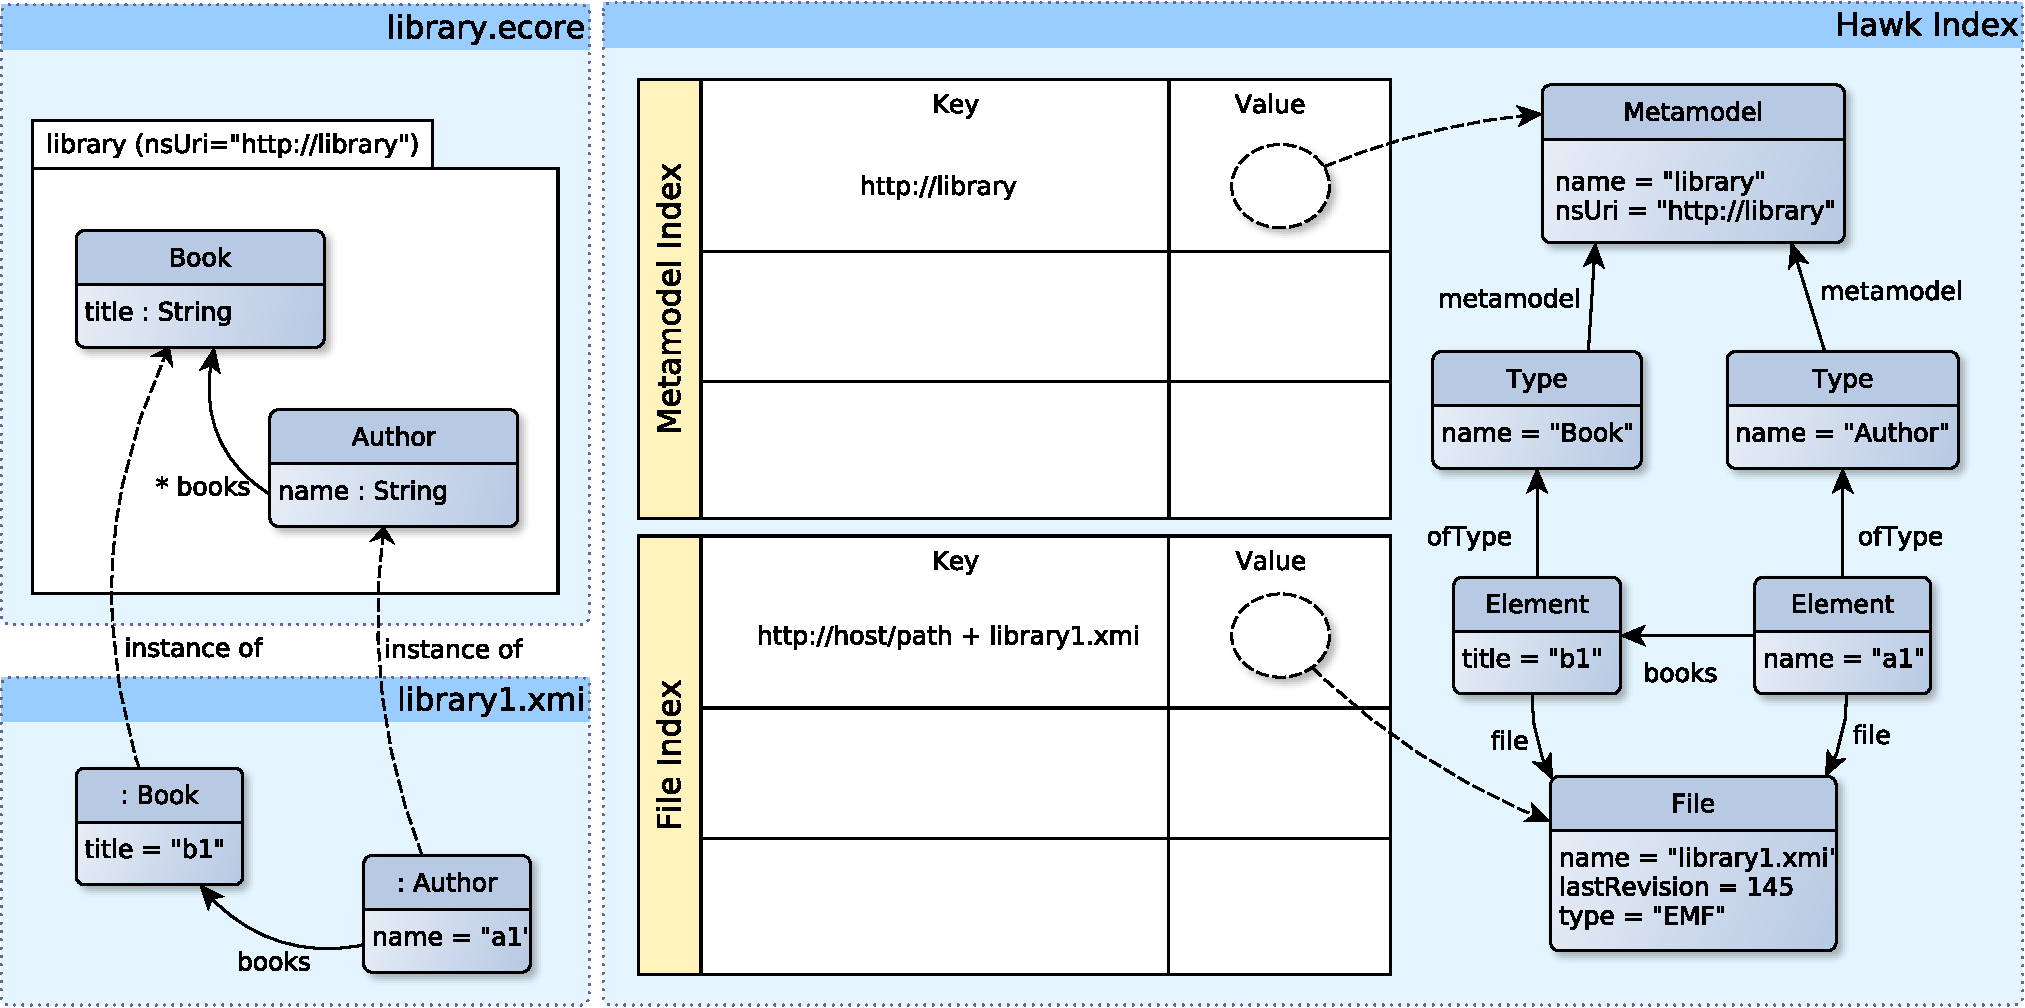
\includegraphics[width=\textwidth]{hawk-library-cropped}
  \begin{overprint}
    \onslide<1>
    \begin{tikzpicture}[remember picture,overlay]
      \draw[fill=white,fill opacity=0.8,draw=none]
      (page cs:-0.345,-0.4) rectangle (page cs:0.9,0.78);
    \end{tikzpicture}
    \begin{center}
      We go from these model files...
    \end{center}

    \onslide<2>
    \begin{tikzpicture}[remember picture,overlay]
      \draw[fill=white,fill opacity=0.8,draw=none]
        (page cs:-1.0,0.78) rectangle (page cs:-0.345,-0.4);
    \end{tikzpicture}
    \begin{center}
      ... to these NoSQL graphs.
    \end{center}

    \onslide<3>
    \begin{tikzpicture}[remember picture,overlay,every node/.style={draw=red,very thick},every edge/.style={draw=red,very thick,->}]
      %\printtikzpagegrid
      % \node[minimum width=2em,minimum height=.8em] (nbook) at (page cs:-.675,.405) {};
      % \node[minimum width=6.5em,minimum height=.9em] (nlibrary) at (page cs:-.65,.53) {};
      % \node[minimum width=2em,minimum height=.8em] (nauthor) at (page cs:-.515,.205) {};
      % \node[minimum width=2em,minimum height=.8em] (nbooki) at (page cs:-.71,-.19) {};
      % \node[minimum width=2em,minimum height=.8em] (nauthori) at (page cs:-.47,-.29) {};
      % \node[minimum width=3em,minimum height=.8em] (nmetamodel) at (page cs:.57,.57) {};
      % \node[minimum width=2em,minimum height=.8em] (nbookt) at (page cs:.44,.27) {};
      % \node[minimum width=2em,minimum height=.8em] (nauthort) at (page cs:.695,.27) {};
      % \node[minimum width=2em,minimum height=.8em] (nbooke) at (page cs:.435,.02) {};
      % \node[minimum width=2em,minimum height=.8em] (nauthore) at (page cs:.695,.02) {};
      % \node[minimum width=2em,minimum height=.8em] (nfile) at (page cs:.57,-.2) {};
      % \node[minimum width=6.5em,minimum height=.8em] (nmetamodelkey) at (page cs:-.062,.485) {};
      % \node[minimum width=6.5em,minimum height=.8em] (nfilekey) at (page cs:-.062,-.015) {};
      % \path
      %   (nlibrary) edge[out=0,in=180] (nmetamodel)
      %   (nbook) edge[out=0,in=180] (nbookt)
      %   (nauthor) edge[out=0,in=200] (nauthort);

      \draw[fill=white,fill opacity=0.8,draw=none]
        (page cs:-0.9,-.4) rectangle (page cs:-.35,.02);
      \draw[fill=white,fill opacity=0.8,draw=none]
        (page cs:-0.345,-.4) rectangle (page cs:0.34,0.78);
      \draw[fill=white,fill opacity=0.8,draw=none]
        (page cs:0.34,-.4) rectangle (page cs:0.85,0.15);
    \end{tikzpicture}
    \begin{itemize}
    \item Ecore packages $\rightarrow$ metamodel nodes
    \item Ecore classes $\rightarrow$ type nodes
    \end{itemize}

    \onslide<4>
    \begin{tikzpicture}[remember picture,overlay]
      \draw[fill=white,fill opacity=0.8,draw=none]
        (page cs:-.35,.02) rectangle (page cs:-0.9,.78);
      \draw[fill=white,fill opacity=0.8,draw=none]
        (page cs:-0.345,-0.4) rectangle (page cs:0.34,0.78);
      \draw[fill=white,fill opacity=0.8,draw=none]
        (page cs:0.85,0.15) rectangle (page cs:0.34,0.78);
    \end{tikzpicture}
    \begin{itemize}
    \item Physical files $\rightarrow$ file nodes
    \item Model elements $\rightarrow$ element nodes
    \end{itemize}

    \onslide<5>
    \begin{tikzpicture}[remember picture,overlay]
      \draw[fill=white,fill opacity=0.8,draw=none]
        (page cs:-.35,-.4) rectangle (page cs:-0.9,.78);
      \draw[fill=white,fill opacity=0.8,draw=none]
        (page cs:0.85,-.4) rectangle (page cs:0.34,0.78);
    \end{tikzpicture}
    \begin{itemize}
    \item MM index: package URI $\rightarrow$ metamodel node
    \item File index: file path $\rightarrow$ file node
    \item Users can define custom indices by attribute/expression
    \end{itemize}
  \end{overprint}
\end{frame}

\begin{frame}[standout]
  Demo time!

  Let's index a Java model and find singletons.
\end{frame}

\begin{frame}[fragile]{Hawk: indexed attributes}
  \begin{block}{Finding a type by its name}
    \lstinputlisting[language=EOL]{listings/set0-findByName.txt}
  \end{block}

  \begin{block}{This normally involves...}
    \begin{enumerate}
    \item Iterating over all types
    \item Following the ``name'' reference
    \item Comparing the name
    \end{enumerate}
  \end{block}

  \begin{alertblock}{Hawk can replace this with a lookup}
    We only need to tell it to index ``SimpleName.identifier'':
    \lstinputlisting[language=EOL]{listings/set0-findByName-indexed.txt}
  \end{alertblock}
\end{frame}

\begin{frame}[fragile]{Hawk: derived attributes}
  \begin{block}{Original query for finding singletons}
    \lstinputlisting[language=EOL]{listings/singletons.txt}
  \end{block}

  \begin{block}{Can we do it faster?}
    \begin{itemize}
    \item Checking if a method is public or static requires traversing
      references
    \item Same goes for checking if it returns an instance of itself
    \item In Hawk, \alert{we can precompute this}
    \item When files change, only the affected values are recomputed
    \end{itemize}
  \end{block}
\end{frame}

\begin{frame}[fragile]{Hawk: use of derived attributes as precomputed values}

  \begin{block}{Original query}
    \lstinputlisting[language=EOL]{listings/singletons.txt}
  \end{block}

  \begin{block}{Changed to use derived attributes on MethodDeclaration}
    \lstinputlisting[language=EOL,firstline=13]{listings/singletons-dmethods.txt}
  \end{block}
\end{frame}

\begin{frame}{Hawk: derived attributes are also indexed}
  \begin{block}{Revised query}
    \lstinputlisting[language=EOL,firstline=13]{listings/singletons-dmethods.txt}
  \end{block}

  \begin{block}{Can we do it faster?}
    \begin{itemize}
    \item Right now, we need to go through \emph{all} type declarations and then
      filter by methods
    \item What if we go from the methods to the types instead?
    \item In Hawk, \alert{top-level selects can replace iteration with lookups
      when using derived attributes}
    \end{itemize}
  \end{block}
\end{frame}

\begin{frame}{Hawk: use of derived attributes as index keys}

  \begin{block}{Previous query}
    \lstinputlisting[language=EOL,firstline=13]{listings/singletons-dmethods.txt}
  \end{block}

  \begin{block}{Revised to use index, by using derived attributes at the top level}
    \lstinputlisting[language=EOL]{listings/singletons-dmethodsindexed.txt}
  \end{block}

\end{frame}

\begin{frame}[fragile]{Hawk: flagging singletons directly}
  \begin{block}{Previous query}
    \lstinputlisting[language=EOL]{listings/singletons-dmethodsindexed.txt}
  \end{block}

  \begin{block}{Can we do it faster?}
    \begin{itemize}
    \item We could just flag types that are singletons
    \item This derived attribute might be less reusable, however
    \end{itemize}
  \end{block}
\end{frame}

\begin{frame}[fragile]{Hawk: final query for finding singletons}
  \begin{block}{Previous query}
    \lstinputlisting[language=EOL]{listings/singletons-dmethodsindexed.txt}
  \end{block}

  \begin{block}{Final query}
    \lstinputlisting[language=EOL,firstline=12]{listings/singletons-dtypes.txt}
  \end{block}
\end{frame}

\begin{frame}[standout]
  Demo time!

  This time, we will show how to use indexed and derived attributes.
\end{frame}

\begin{frame}[fragile]{Derived edges}
  \begin{block}{Toy example: Person metamodel}
    \begin{itemize}
    \item Person metamodel, with ``parent'' references.
    \item We want to be able to quickly find siblings, grandparents,
      uncles/aunts, cousins, second-cousins, ancestors...
    \item We can precompute this in Hawk with \alert{derived edges}
    \end{itemize}
  \end{block}

  \begin{block}{Derivation logic for ``grandparent''}
    We need a flat list and not a list of lists, so we use ``flatten'':
    \begin{lstlisting}[language=EOL]
      return self.parent.parent.flatten;
    \end{lstlisting}
  \end{block}

  \begin{block}{Derivation logic for ``sibling''}
    We can travel references in reverse with ``revRefNav\_name'':

    \begin{lstlisting}[language=EOL]
      return self.parent.revRefNav_parent.flatten.excluding(self);
    \end{lstlisting}
  \end{block}

\end{frame}

\begin{frame}[standout]
  Last demo for Hawk.

  We will show derived edges this time.
\end{frame}

\begin{frame}{Hawk: integration into SOFTEAM Constellation~\cite{hawkmodelio_2016}}

  \centering
  \begin{columns}
    \column{.5\textwidth}
    \begin{center}
  \resizebox{\columnwidth}{!}{
    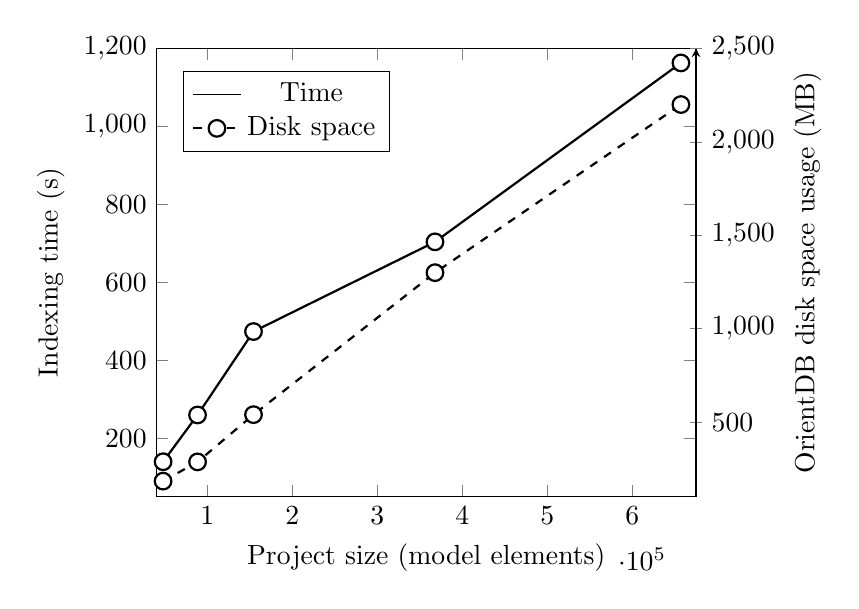
\begin{tikzpicture}
      \begin{axis}[
        xlabel={Project size (model elements)},
        ylabel={Indexing time (s)},
        xmin=40000,xmax=675000,
        ymin=50,ymax=1200
        ]
        \addplot+[black,thick,mark options={solid,mark size=3,fill=white}] coordinates {
          (47891, 140)
          (88451, 260)
          (154281, 474)
          (367840, 704)
          (657228, 1163)
        }; \label{Hplot}
      \end{axis}
      \begin{axis}[
        axis x line=none,
        axis y line=right,
        ylabel={OrientDB disk space usage (MB)},
        xmin=40000,xmax=675000,
        ymin=100,ymax=2500,
        legend style={at={(0.05,0.95)},anchor=north west}
        ]
        \addlegendimage{/pgfplots/refstyle=Hplot}\addlegendentry{Time}
        \addplot+[black,thick,dashed,mark options={solid,mark size=3,fill=white}] coordinates {
          (47891, 184)
          (88451, 287)
          (154281, 540)
          (367840, 1300)
          (657228, 2200)
        }; \addlegendentry{Disk space}
      \end{axis}
    \end{tikzpicture}
  }
  \textbf{Indexing times and index sizes (OrientDB backend)}
\end{center}


    \column{.4\textwidth}
    \begin{center}
  \resizebox{\columnwidth}{!}{
    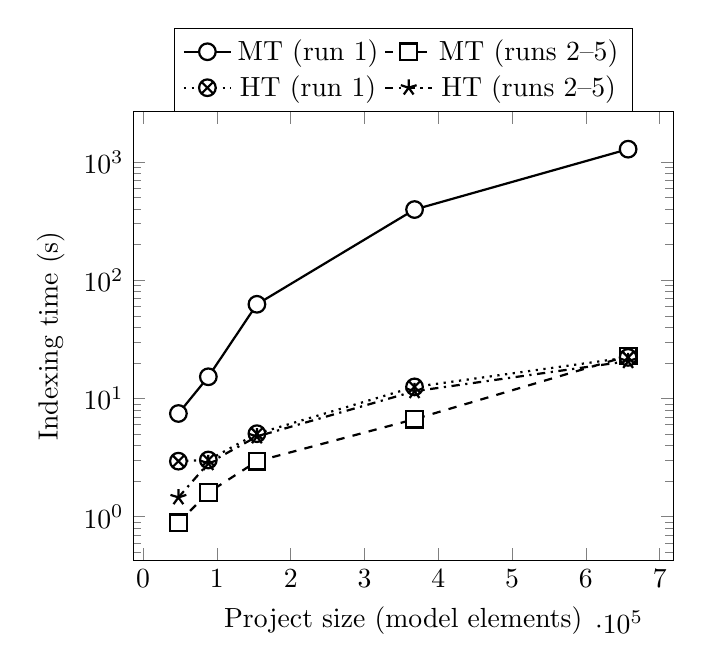
\begin{tikzpicture}
      \begin{semilogyaxis}[
        xlabel={Project size (model elements)},
        ylabel={Indexing time (s)},
        legend entries={
          {MT (run 1)},
          {MT (runs 2--5)},
          {HT (run 1)},
          {HT (runs 2--5)}
        },
        legend style={
          legend columns=2,
          at={(0.5,1)},
          anchor=south,
        },
        mark options={solid,mark size=3},
        ]
        \addplot+[black,thick,mark options={solid,mark size=3,fill=white}] coordinates {
          (47891, 7.465)
          (88451, 15.260)
          (154281, 62.550)
          (367840, 395.659)
          (657228, 1281.042)
        };
        \addplot+[black,thick,dashed,mark options={solid,mark size=3,fill=white}] coordinates {
          (47891, 0.890)
          (88451, 1.604)
          (154281, 2.944)
          (367840, 6.682)
          (657228, 22.891)
        };
        \addplot+[black,thick,dotted,mark options={solid,mark size=3,fill=white}] coordinates {
          (47891, 2.951)
          (88451, 3.019)
          (154281, 5.039)
          (367840, 12.531)
          (657228, 22.247)
        };
        \addplot+[black,thick,dashdotted] coordinates {
          (47891, 1.457)
          (88451, 2.834)
          (154281, 4.771)
          (367840, 11.510)
          (657228, 20.661)
        };
      \end{semilogyaxis}
    \end{tikzpicture}
  }
  \textbf{Code generation times: Modelio (MT), Hawk (HT)}
\end{center}

  \end{columns}

  \begin{itemize}
  \item Constellation: collaboration platform over Modelio models
  \item SOFTEAM needed search, couldn't change persistence
  \item Integrated Hawk as a library: initial indexing cost quickly paid off
  \end{itemize}
\end{frame}

\begin{frame}{Hawk: stress-testing remote query APIs~\cite{sosym-stress-2017}}

  \begin{center}
    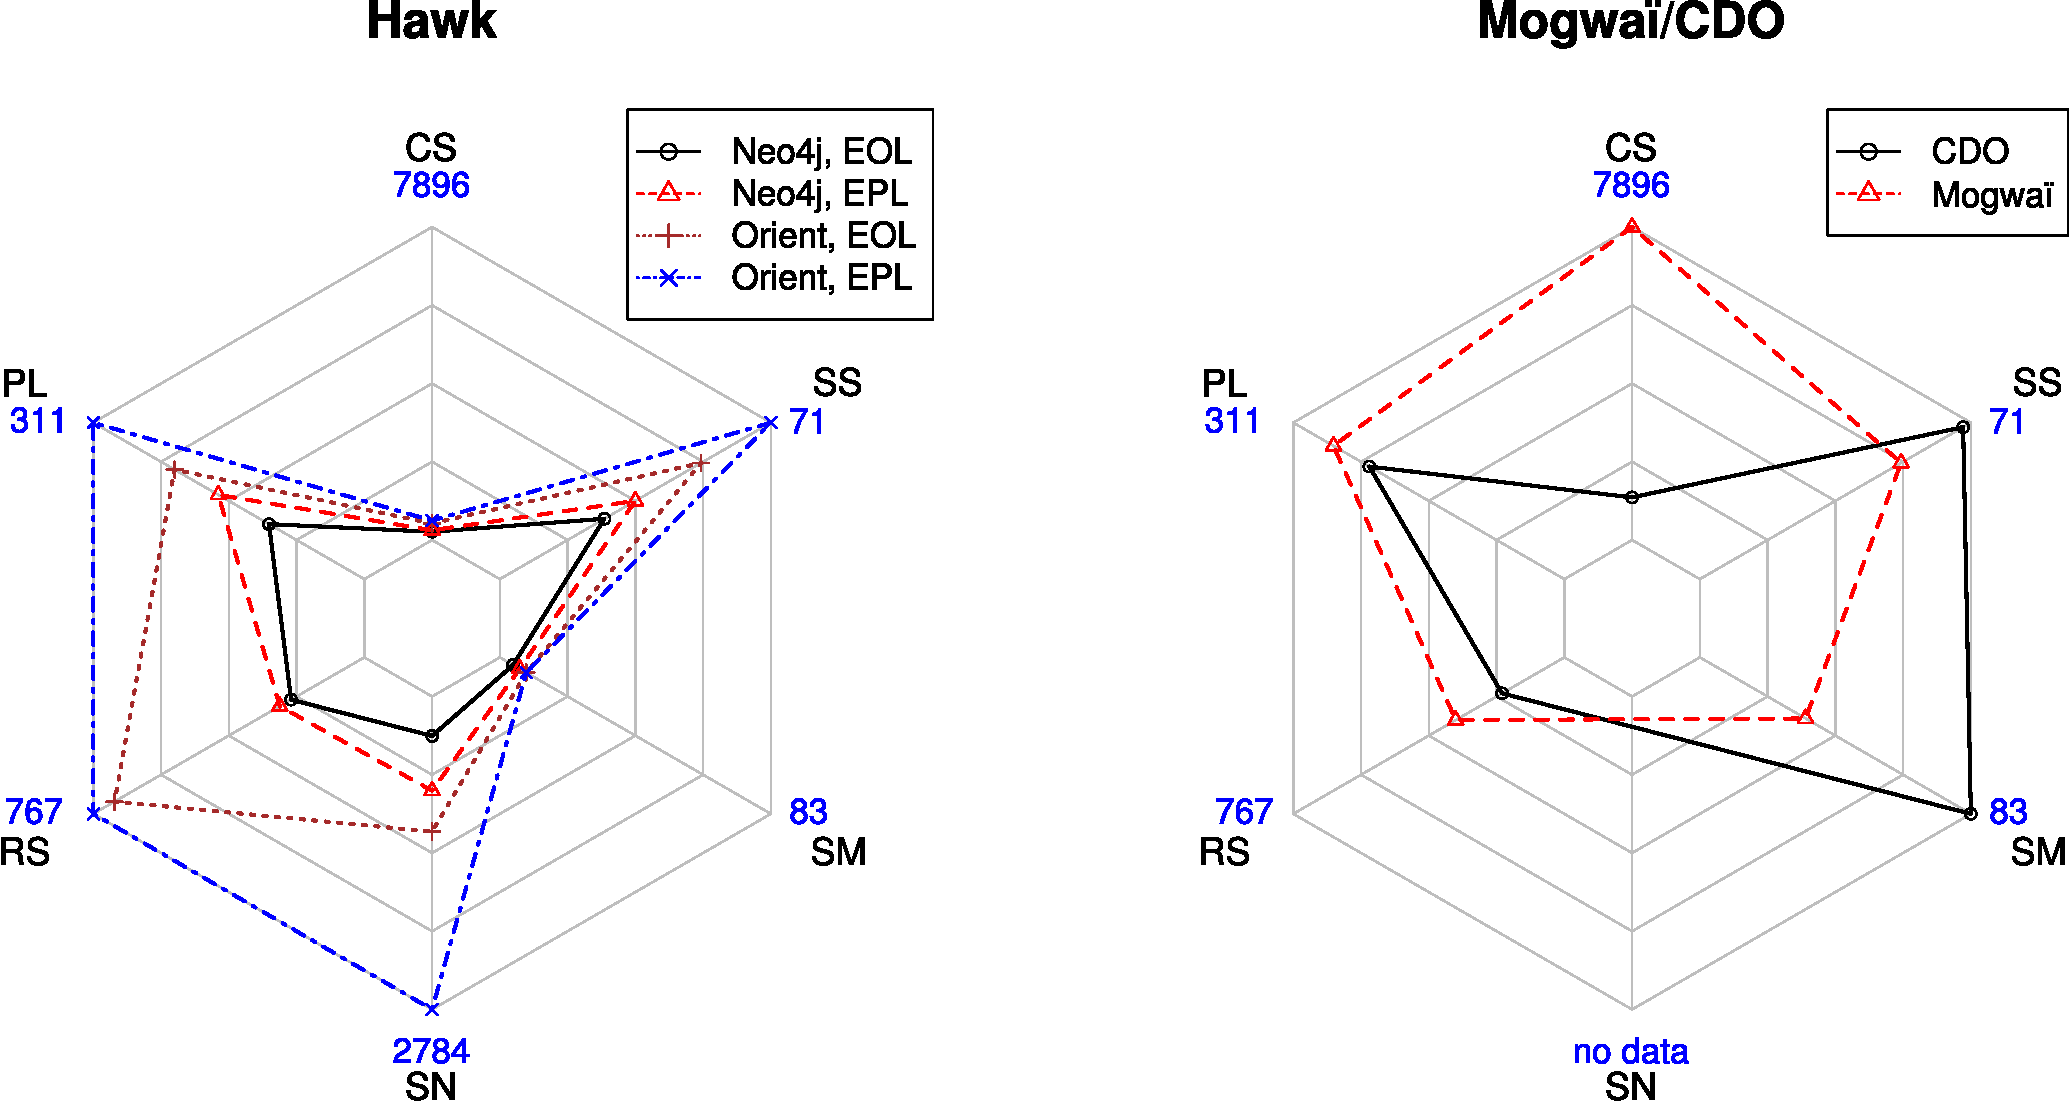
\includegraphics[width=\textwidth]{rq3-comparison-tb}
  \end{center}

  \begin{itemize}
  \item Included CDO, Hawk, Mogwaï and ranged 1--64 clients
  \item Reverse reference navigation was crucial in having the
    SN Train Benchmark~\cite{trainbenchmark} query run quickly
  \end{itemize}

\end{frame}

\begin{frame}{Hawk: summing up}

  \begin{block}{So far...}
    \begin{itemize}
    \item Hawk is good for indexing an existing collection of model files
    \item You can efficiently answer queries from the index
    \item Indexed/derived features can be used to speed up queries
    \end{itemize}
  \end{block}

  \begin{block}{Ideas in the roadmap}
    \begin{itemize}
    \item Extensible UI: right now it's prefixed
    % Folding Space immediately asked about horizontal scaling, interestingly
    \item Horizontal scaling (a flock of Hawks?)
    \item Temporal querying:
      \begin{itemize}
      \item When did this graph pattern match happen?
      \item What happened before/after?
      \end{itemize}
    \item Web UI, based on Thrift API
    \end{itemize}

    Feedback and contributions are welcome!
  \end{block}

\end{frame}

\section{NeoEMF}

\begin{frame}[t]\frametitle{NeoEMF: Architecture}
    \begin{center}
      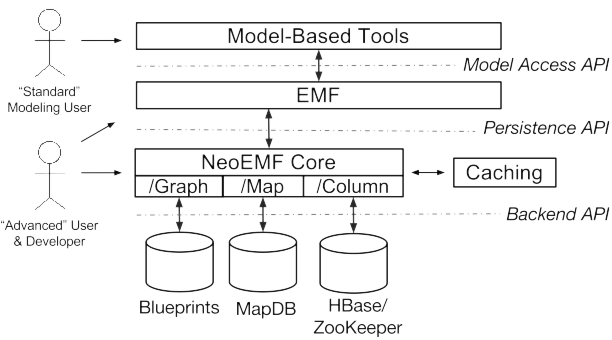
\includegraphics[width=\textwidth]{neoemf-architecture.png}
    \end{center}
\end{frame}

\begin{frame}[t]\frametitle{NeoEMF: project website}
    \begin{center}
      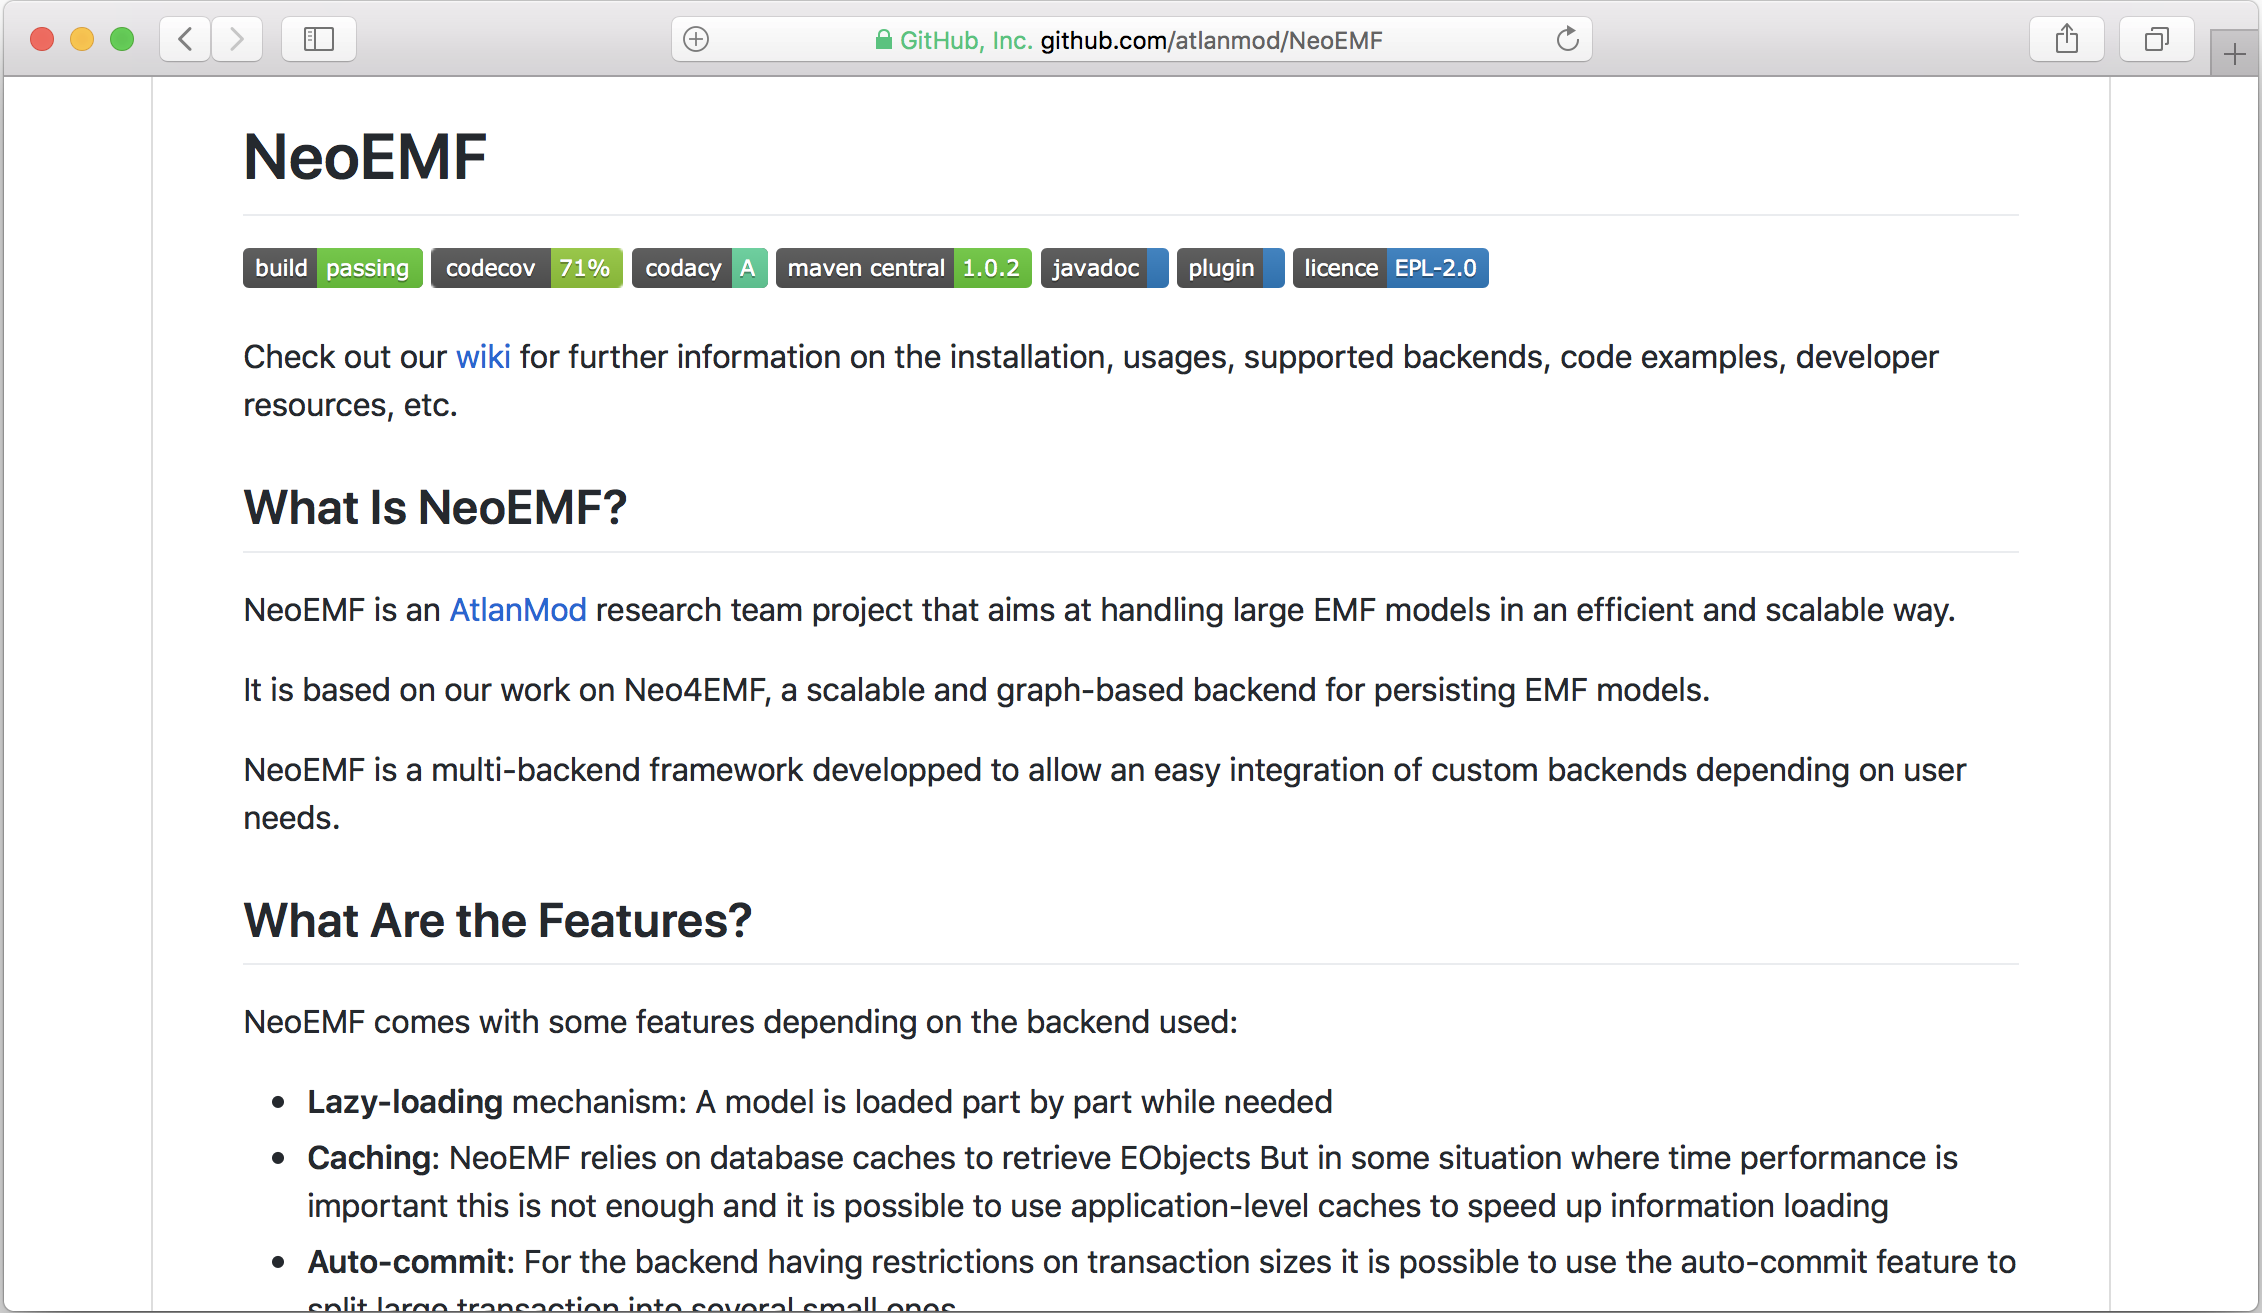
\includegraphics[width=\textwidth]{neoemf-github.png}
    \end{center}
	
    \begin{itemize}
    \item \url{https://github.com/atlanmod/NeoEMF}
    \item Open source project under the Eclipse Public License 2.0
    \end{itemize}
\end{frame}

\begin{frame}[c]\frametitle{NeoEMF Datastores~\cite{DBLP:conf/models/DanielSBTVGC16}}
	\begin{itemize}
		\item NeoEMF/Graph
		\begin{itemize}
			\item Efficient model traversal using rich query language
			\item Mogwaï framework (OCL to Gremlin translation)
		\end{itemize}
		\item NeoEMF/Map
		\begin{itemize}
			\item Fast access to atomic operations
			\item Designed for EMF-API calls
		\end{itemize}
		\item NeoEMF/Column
		\begin{itemize}
			\item Transparent model distribution
			\item Concurrent read/write
			\item Distributed model transformations (ATL-MR)
		\end{itemize}
	\end{itemize}
\end{frame}

\begin{frame}[c]\frametitle{NeoEMF Key Features}
	\begin{itemize}
		\item Lazy-loading
		\item Compliant with EMF API
		\item Easy to integrate in existing applications
		\item EMF-Compatible code generation
		\item Advanced caching (+ prefetching) strategies
		\item Efficient XMI importer
	\end{itemize}
\end{frame}

\begin{frame}[fragile]\frametitle{Initialise a New Resource}
	\begin{enumerate}
		\item Create a new URI to locate a file-based resource.
		\item Create the resource.
	\end{enumerate}
	
\begin{java}
URI uri = MyUriBuilder.builder().fromFile(new File("<db_path>"));

ResourceSet resourceSet = new ResourceSetImpl();
Resource resource = resourceSet.createResource(uri);
\end{java}
\end{frame}

\begin{frame}[fragile]\frametitle{Save/Load Resource}
	
	\begin{enumerate}
		\item Create a new configuration builder.
		\item Save and unload resource.
	\end{enumerate}
\begin{java}
ImmutableConfig config = MyConfig.newConfig()
  .autoSave(50000)              
  .log()                        
  .withOption("key", "value");  

resource.load(config.asMap()); 

// Do something on the resource

resource.save(config.asMap()); 
resource.unload();
\end{java}
	
\end{frame}

\begin{frame}[fragile]\frametitle{Modify existing resource}
	\begin{enumerate}
		\item Load resource.
		\item Modify contents.
		\item Save resource. 
	\end{enumerate}
	
\begin{java}
ImmutableConfig config = MyConfig.newConfig()
  .cacheContainers()
  .cacheMetaclasses();

URI uri = MyUriBuilder.builder().fromFile(new File("db_path"));

Resource resource = new ResourceSetImpl().createResource(uri);
resource.load(config.asMap());

MyClass myClass = (MyClass) resource.getContents().get(0);
myClass.setName("NewName");

resource.save(config.asMap());
resource.unload();
\end{java}
\end{frame}

\begin{frame}[standout]
  Demo time!

  Let's import a Java model, save it in Neo4j and query the database.
\end{frame}

\begin{frame}[c]\frametitle{Discussion}
	\begin{itemize}
		\item Graph databases outperform relational ones for several navigation steps queries.
		\item But model loading operations only use 2 or 3 steps queries.
		\item If the use of the EMF API is the only concern, then a relational (or column) database storing BLOBs are a better solution.
		\item Impossible to compare with bigger models.
	\end{itemize}
\end{frame}

\begin{frame}[c]\frametitle{Discussion}
    \begin{center}
      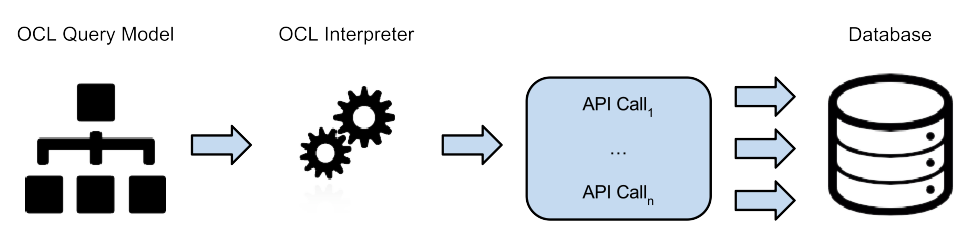
\includegraphics[width=\textwidth]{neoemf-discussion.png}
    \end{center}
	\begin{itemize}
		\item Low-level model handling APIs
		\item Fragmented queries on the database
		\item Many intermediate objects
	\end{itemize}
\end{frame}

\section{Mogwa\"i}

\begin{frame}[c]\frametitle{Motivation}
	\begin{itemize}
		\item Why don't we query directly the database?
		\item Manually writing database-level queries is hard
		\item Need to learn a new query language
		\item Database expertise vs. Modeling expertise
		\item Unknown model representation
		\item Solution: generate them!
	\end{itemize}
	
\end{frame}

\begin{frame}[t]\frametitle{Mogwa\"i: Architecture~\cite{DBLP:conf/rcis/DanielSC16}}
    \begin{center}
      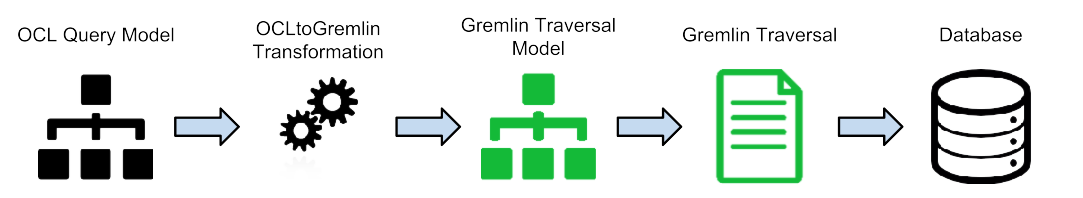
\includegraphics[width=\textwidth]{mogwai-architecture.png}
    \end{center}
	\begin{itemize}
		\item Generate graph database queries from OCL expressions
		\item Bypass modelling framework API
		\item Single execution of the query
	\end{itemize}
	
\end{frame}

\begin{frame}[c]\frametitle{Mogwa\"i: project website}
    \begin{center}
      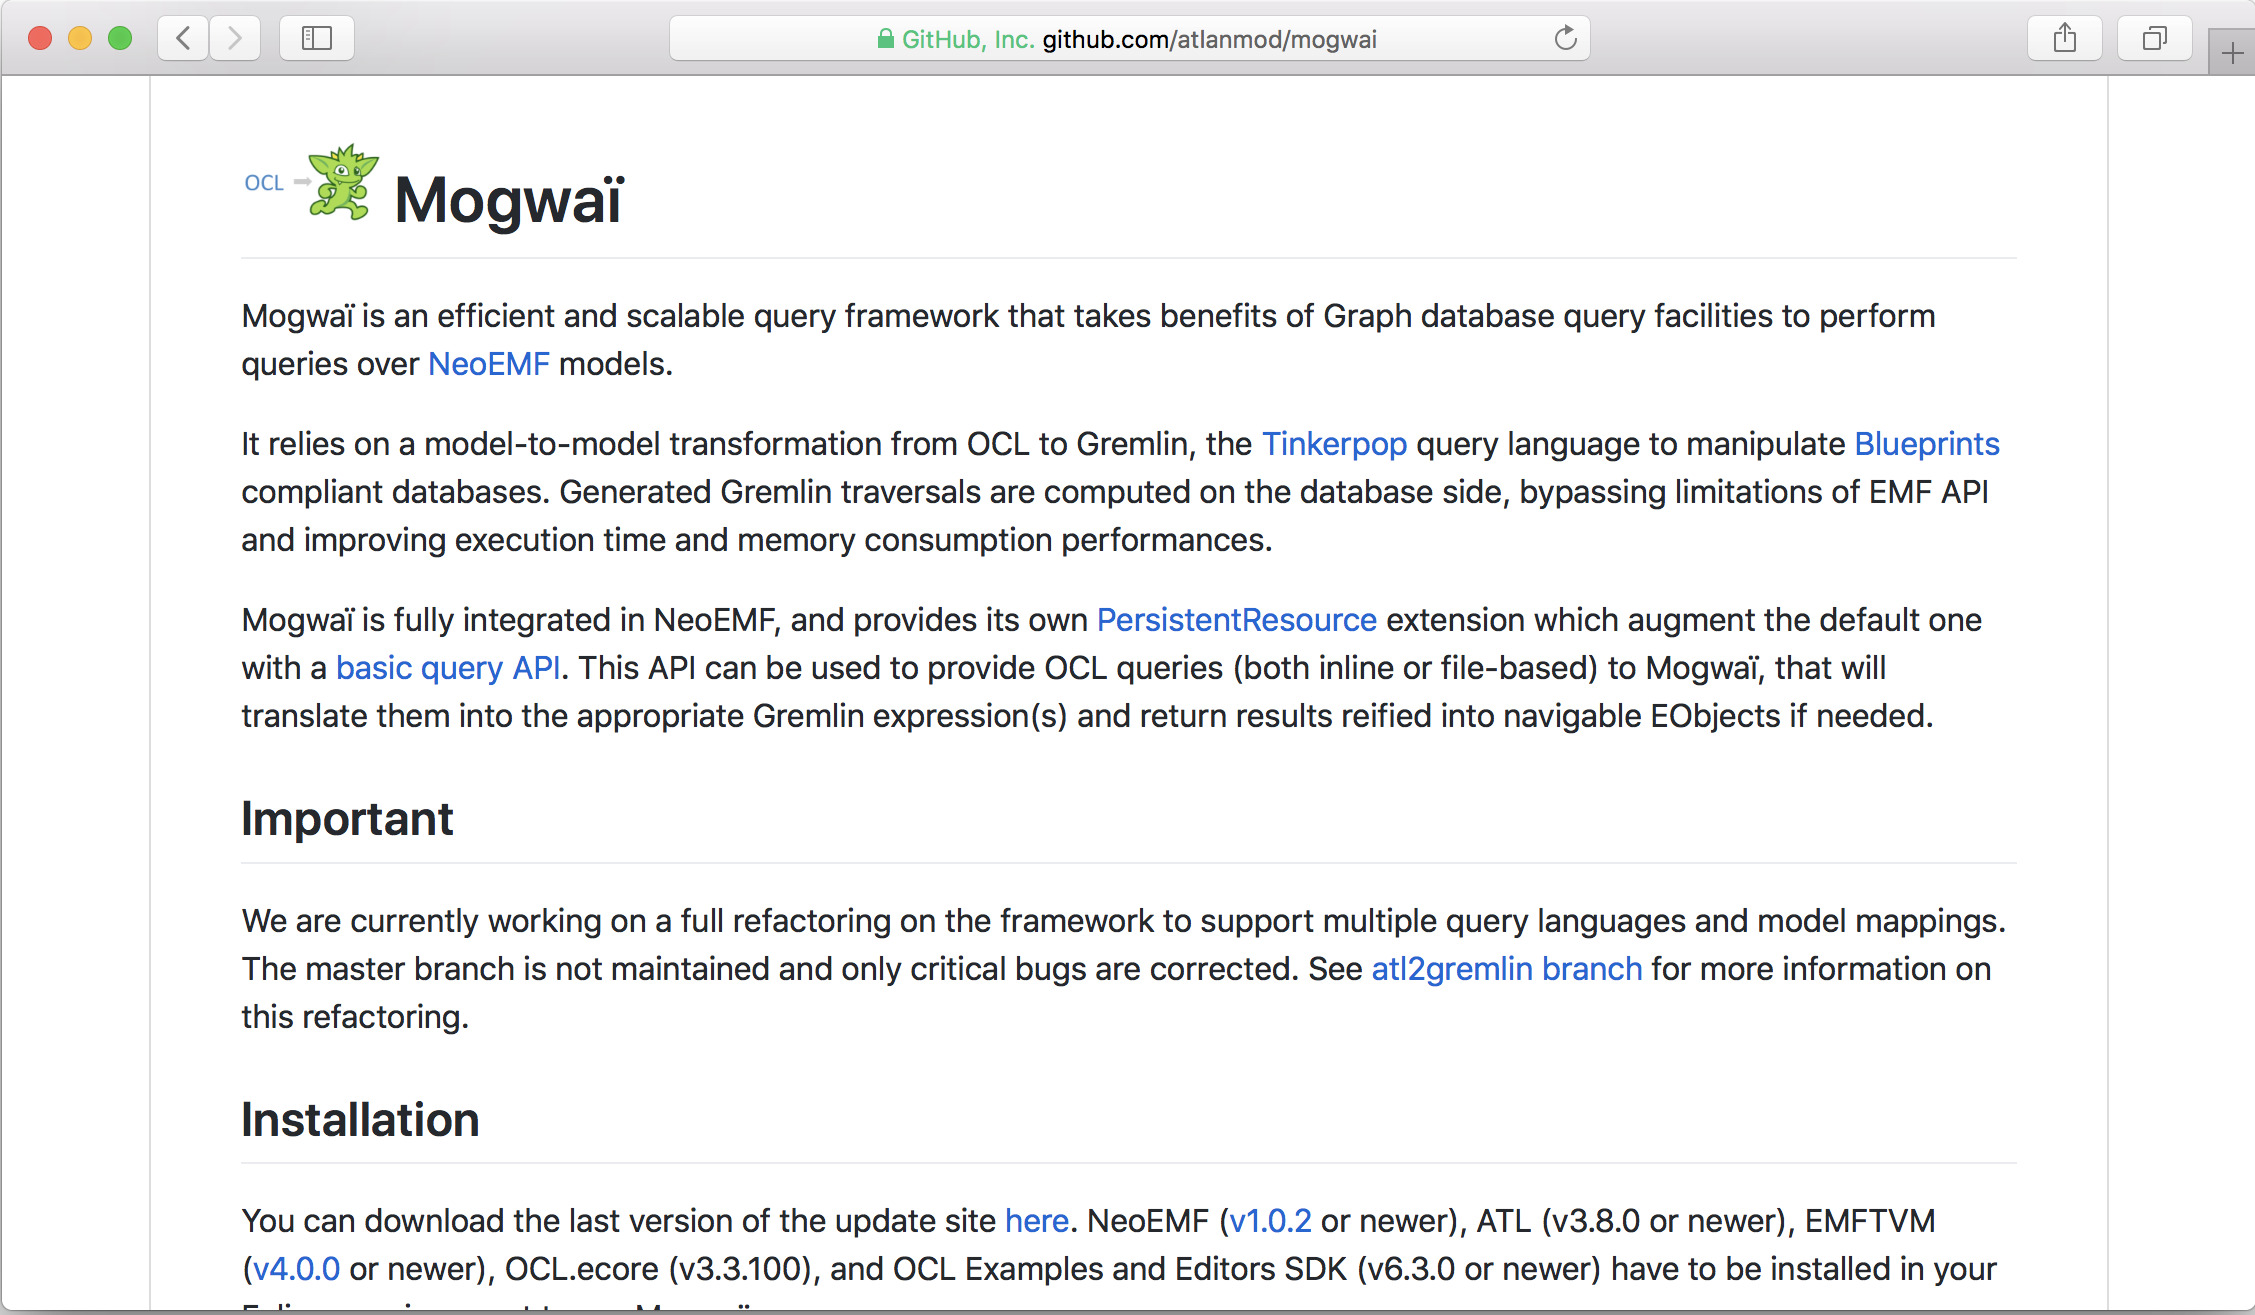
\includegraphics[width=\textwidth]{mogwai-github.png}
    \end{center}
	
    \begin{itemize}
    \item \url{https://github.com/atlanmod/mogwai}
    \item Open source project under the Eclipse Public License 2.0
    \end{itemize}
\end{frame}

\begin{frame}[fragile]\frametitle{Queries are expressed in OCL}
	
	\begin{columns}
		\begin{column}{0.5\textwidth}
	\begin{figure}[htbp]
		\centering
			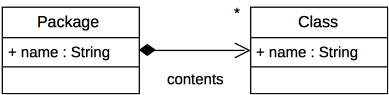
\includegraphics[width=\textwidth]{mogwai-model.png}
		\caption{Simple Model}
		\label{fig:label}
	\end{figure}
	\begin{figure}[htbp]
		\centering
			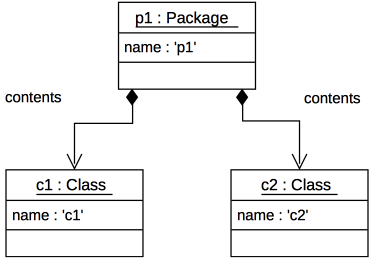
\includegraphics[width=\textwidth]{mogwai-instances.png}
		\caption{Model Instances}
		\label{fig:label}
	\end{figure}		
		\end{column}
		\begin{column}{0.5\textwidth}
		\begin{ocl}
Package.allInstances()  -- returns p1
p1.contents				-- returns [c1,c2]
p1.contents->select(e | e.name = 'c1') 
		-- returns c1
		\end{ocl}
		\end{column}
	\end{columns}
\end{frame}

\begin{frame}[c]\frametitle{Model Persistence}
	\begin{figure}[htbp]
		\centering
			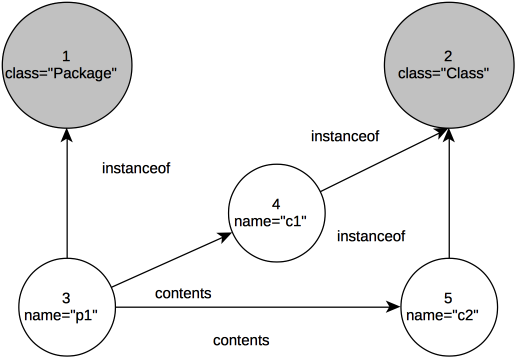
\includegraphics[width=.6\linewidth]{mogwai-graph.png}
		\caption{Model Instances Stored in Neo4j}
		\label{fig:label}
	\end{figure}
\end{frame}

\begin{frame}[fragile]\frametitle{Database Queries are expressed in Gremlins}
	\begin{itemize}
		\item Graph traversal DSL
		\item Composed of processing steps
		\item Generic query language for graph databases
	\end{itemize}
	\begin{columns}
		\begin{column}{0.4\textwidth}
			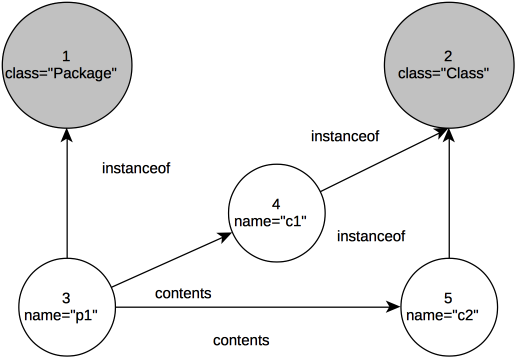
\includegraphics[width=\linewidth]{mogwai-graph.png}
		\end{column}
		\begin{column}{0.6\textwidth}
\begin{lstlisting}[language=gremlin]
g.idx(''metaclasses'')[[name:''Package'']]
    .inE(''instanceOf'').outV // v(1)
g.v(3).outE(''contents'').inV // [v(4),v(5)]
g.v(3).outE(''contents'').inV
    .filter{it.name = ''c1''} // v(4)
\end{lstlisting}
		\end{column}
	\end{columns}
	
\end{frame}

\begin{frame}[c]\frametitle{OCL Queries into Gremlin Traversals Translation}
	\begin{itemize}
		\item Map OCL expressions to Gremlin steps
		\item Merge created steps into a (several) traversal(s)]
	\end{itemize}
    \begin{center}
      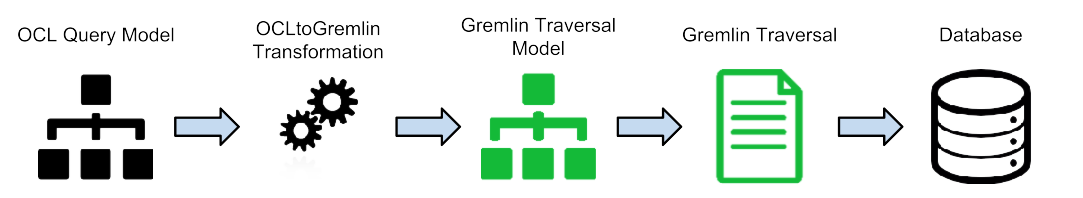
\includegraphics[width=\textwidth]{mogwai-architecture.png}
    \end{center}	
\end{frame}

\begin{frame}[c]\frametitle{OCL Expressions to Gremlin Steps Mapping}
	\begin{columns}
		\begin{column}{0.5\textwidth}
    \begin{center}
      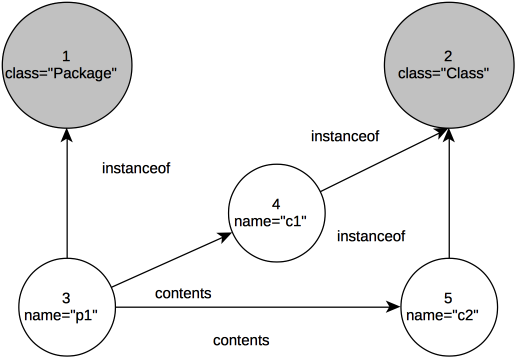
\includegraphics[width=\textwidth]{mogwai-graph.png}
    \end{center}			
		\end{column}
		\begin{column}{0.5\textwidth}
    \begin{center}
      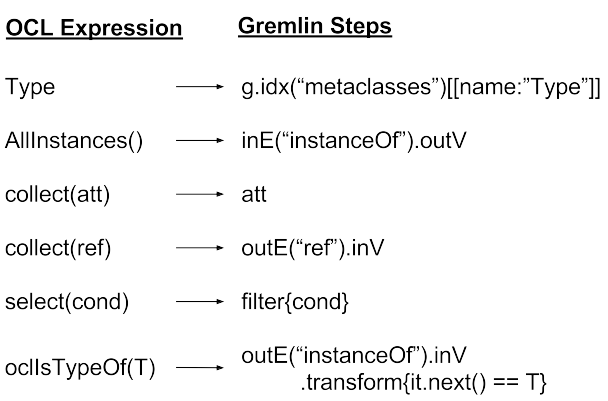
\includegraphics[width=\textwidth]{mogwai-mapping.png}
    \end{center}			
		\end{column}
	\end{columns}
\end{frame}

\begin{frame}[c]\frametitle{Merge created steps into a traversal}
    \begin{center}
      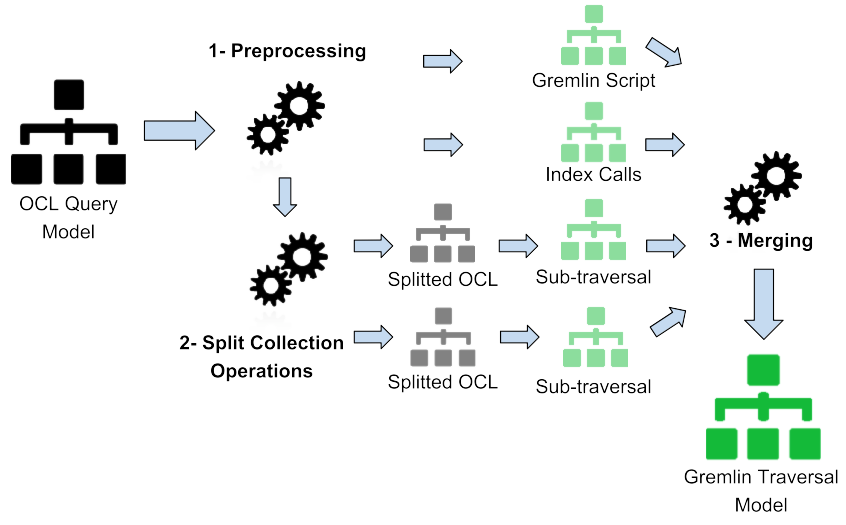
\includegraphics[width=\textwidth]{mogwai-transformation.png}
    \end{center}
\end{frame}

\begin{frame}[c]\frametitle{OCL Transformation Example}
    \begin{center}
      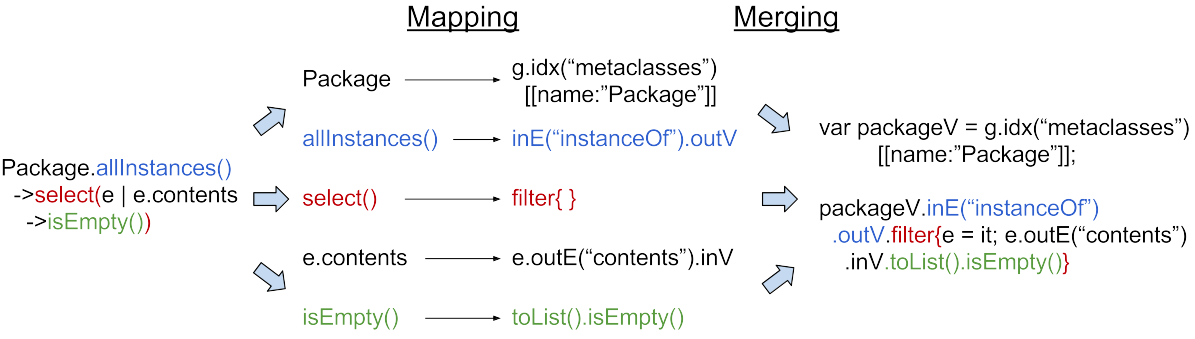
\includegraphics[width=\textwidth]{mogwai-ocl-transformation.png}
    \end{center}	
\end{frame}

\begin{frame}[c]\frametitle{Query generation and execution}
	
	\begin{itemize}
		\item Delegates query computation to the database
		\item Returns graph elements to the persistence layer
	\end{itemize}
	
 \begin{center}
   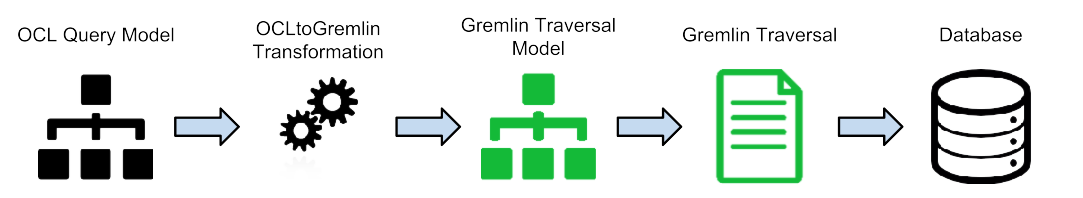
\includegraphics[width=\textwidth]{mogwai-architecture.png}
 \end{center}
	
\end{frame}

\begin{frame}[standout]
  Demo time!

  Let's query a Java model and find singletons.
\end{frame}

\begin{frame}[c]\frametitle{Benchmark Results}
\begin{itemize}
	\item Model containing 2 million elements
	\item Up to 20 times faster than other query approaches
	\item Consume up to 75 times less memory
\end{itemize}
\begin{columns}
	\begin{column}{0.5\textwidth}
	    \begin{center}
	      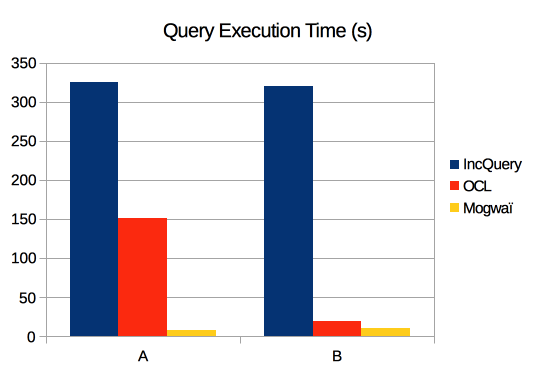
\includegraphics[width=\textwidth]{mogwai-benchmark-cpu.png}
	    \end{center}
	\end{column}
	\begin{column}{0.5\textwidth}
	    \begin{center}
	      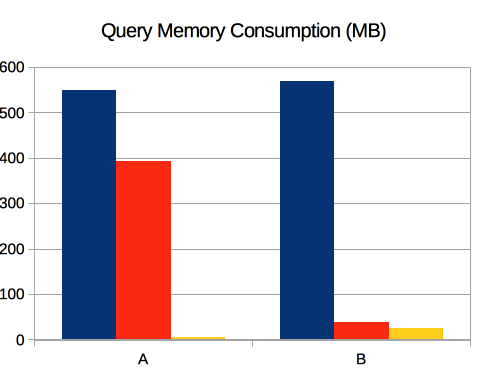
\includegraphics[width=\textwidth]{mogwai-benchmark-memory.png}
	    \end{center}
	\end{column}
\end{columns}


\end{frame}

\begin{frame}[c]\frametitle{Conclusion}
	\begin{block}{Model Persistence Frameworks}
	\begin{itemize}
		\item Not designed to compute model queries efficiently
		\item Writing manually database-level queries is hard
	\end{itemize}
	\end{block}

\begin{block}{Mogwaï}
		\begin{itemize}
		\item Translates OCL queries into Gremlin traversals
		\item Positive results
		\item Not adapted to small models
		\item Needs to be integrated
	\end{itemize}
\end{block}
\end{frame}


\section{Wrap-up}

\begin{frame}{Summary}

  \begin{block}{Use cases}
    \begin{itemize}
    \item For fast querying with no changes to persistence: Hawk
    \begin{itemize}
    \item Make sure your models are fragmented
    \item Hawk will only re-index the changed fragments
    \end{itemize}
    \item For scalable storage with no fragmentation: NeoEMF
    \end{itemize}
  \end{block}

  \begin{block}{Feedback and contributions welcome!}
  \begin{itemize}
  \item Hawk, NeoEMF and Mogwaï are all open-source
  \item Chat with us if you have an idea for an application
  \end{itemize}
  \end{block}

\end{frame}

\appendix

{\setbeamercolor{palette primary}{fg=black, bg=yellow}
\begin{frame}[standout]
  Questions?
\end{frame}
}

\begin{frame}[allowframebreaks]{References}

  \bibliography{bibliography}
  \bibliographystyle{alpha}

\end{frame}

\end{document}
